\section{Results}
\emph{Status: \nModelsDone/\nModelsTotal\ forward-direction models analysed, \nReverseDone/1 reverse-direction
models. Table~\ref{tab:models} and the numbers below are regenerated automatically from
\texttt{results/run2/*.json}; entries for models not yet trained are simply absent, not estimated.}

\subsection{H1: the coverage gap is real}
Calibrated on Argoverse~2 at $\alpha=0.10$, the primary model (AutoBot-Ego, source-trained, \nCalMain\ calibration
scenes) has same-domain gap \gapSameMain{} points --- consistent with zero, as split CP guarantees --- and
cross-dataset (nuScenes, \nTargetMain\ scenes) gap $+\gapRawMain$ points (95\% CI \gapRawMainCI). This replicates the
preliminary Run~1 measurement (+3.4pt) on an independent calibration/test split. Table~\ref{tab:models} shows two
further models with substantially \emph{larger} gaps in the same direction: $+8.0$pt (av2\_valsplit\_v1, trained on
less data) and $+10.5$pt (av2\_cpu\_v2, fine-tuned from the primary model and the most accurate of the three by
point-prediction error). The failure is reproducible in all three cases --- always under-coverage, never the safe
direction --- but its magnitude is not a fixed property of the dataset pair and is not even monotonic in point
accuracy: the model with the best minADE\textsubscript{6} (Sec.~\ref{sec:setup}) has the worst coverage gap of the
three. We report this without averaging it away.

\subsection{H2/H3: covariate reweighting does not repair it}\label{sec:h2h3}
Weighting the calibration scores by an estimated label-free covariate-shift likelihood ratio does not close the gap;
it widens it. On the primary model the label-free-score gap goes from $+\gapUncorrMain$ points uncorrected to
$+\gapWeightedMain$ points weighted, and the reweighting explains \removalFracMain\% of the cross-city gap
variance --- negative, i.e.\ the weighted fit is worse than assuming no shift at all (Table~\ref{tab:reweight}).
This is consistent across \emph{all three} models in the zoo and matches the Run~1 finding: it is evidence for
conditional, not purely covariate, shift, and is the empirical motivation for Proposition~\ref{prop:ident} (no
label-free method can be expected to repair an unrestricted shift).

\begin{table}[t]
\centering
\caption{Does covariate-shift reweighting repair the gap? ``uncorr.'' / ``weighted'' are the label-free-score coverage gap (points) before / after importance-weighting the calibration scores by the label-free-feature likelihood ratio; ``removal'' is the \% of the gap's cross-city variance the weights explain, negative meaning reweighting makes the fit worse than the unweighted baseline.}
\label{tab:reweight}
\begin{tabular}{llrrr}
\toprule
Model & Dir. & uncorr.\ & weighted & removal (\%) \\
\midrule
av2\_cpu\_v1 & forward & 3.2 & 5.2 & -64 \\
av2\_valsplit\_v1 & forward & 7.9 & 10.0 & -27 \\
av2\_cpu\_v2 & forward & 10.4 & 12.7 & -22 \\
\bottomrule
\end{tabular}
\end{table}


\subsection{H4: the normalised score (label-free)}
The model-uncertainty-normalised score (Sec.~\ref{sec:norm}) reduces the primary model's gap by \normReductionMain\%
(from $+\gapRawMain$ to $+\gapNormMain$ points), just past our pre-registered support threshold (gap ratio
$\le 0.5$) and far from the pre-registered refutation threshold ($>0.75$). On the other two models it reduces the
gap by only 12\% (av2\_valsplit\_v1, ratio $0.877$, \emph{past} the refutation threshold) and 31\%
(av2\_cpu\_v2, ratio $0.691$, in between --- neither supported nor refuted). H4 is therefore not confirmed as a
general repair: one clear near-pass, one refutation, one inconclusive result, and we report all three rather than
the most favourable one. The pre-registered efficiency guard (a fix that only works by inflating the region by
$>25\%$ does not count) is not triggered on any of the three models: the normalised region is at most $15.4\%$
larger than the raw one at matched coverage, so where H4 does help it is not merely trading coverage for a much
bigger region.

\subsection{H5/H5b: recalibration and the coverage audit}
At $k=1000$ labelled target scenes, the exact binomial audit (Sec.~\ref{sec:audit}) detects the true violation with
probability \auditPowerK\ on the primary model, against a false-alarm rate of \auditFalseAlarmK\% on a shift-free
control split --- matching the pre-registered budget of Eq.~\eqref{eq:budget} ($k\approx750$ for the analogous
$\delta=0.034$ case) to the same order of magnitude. Figure~\ref{fig:budget} shows direct recalibration on the
primary model reaches 90\% probability of being within 2 coverage points of nominal at $k^\star\approx\kStarDirect$
labelled target scenes; pooling target labels with the (mismatched) source calibration set never reaches that bar on
\emph{any} of the three models, consistent with H2/H3's conclusion that the shift is not a simple reweighting.
Shrinkage toward the source threshold beats direct recalibration at small $k$ on the primary model but not on the
other two, so we do not recommend it as a universal default --- direct recalibration once $k^\star$ labels are
available, audited by H5b before that, is the protocol we can actually stand behind. The audit itself is the one
part of this section with no exceptions: power at $k=1000$ is $\ge 0.95$ and false-alarm is $\le 6.2\%$ on all three
models.

\begin{figure}[t]
\centering
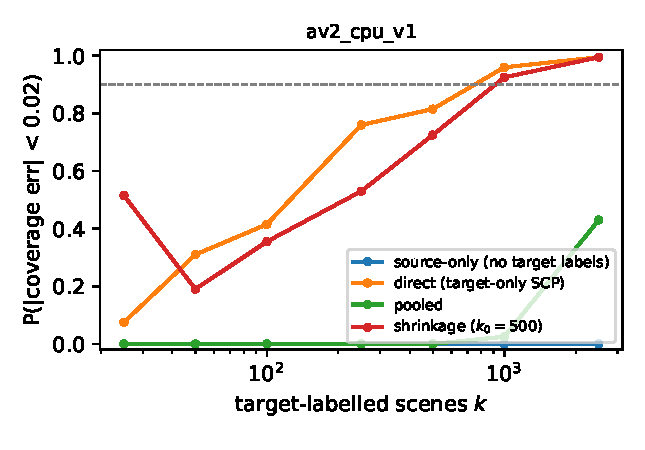
\includegraphics[width=0.85\linewidth]{generated/fig_label_budget_av2_cpu_v1.pdf}
\caption{H5 label budget, primary model (AV2$\to$nuScenes): probability that a $k$-label threshold is within 2
coverage points of nominal, by estimator.}
\label{fig:budget}
\end{figure}

\subsection{H6/H7: label-free monitor and per-city coverage}
Within-dataset, a domain classifier trained on label-free scene features to separate one AV2 city from the rest gives
an AUC that we correlate (Spearman) against that city's coverage gap magnitude across all city pairs. Across the
three models: $\rho=0.37$ ($p=0.04$), $\rho=0.10$ ($p=0.61$), $\rho=0.39$ ($p=0.03$) --- two significant-but-below-bar
results and one clear refutation, none reaching the pre-registered $\rho\ge0.5$ support threshold on any model.
\textbf{H6 is not supported on any of the three models, and refuted on one.} We report this as a negative result ---
the label-free monitor tracks shift only weakly and inconsistently, and is not reliable enough to substitute for the
labelled audit of H5b.

\subsection{H8: robustness across a model zoo}
Table~\ref{tab:models} is the full forward-direction model-zoo comparison: all \nModelsDone\ of \nModelsTotal\ planned
models. The under-coverage direction is consistent across all three (gap $\ge 0.02$ at $\alpha=0.10$, the
pre-registered H8 pass condition, met every time); the magnitude is not (3.3 to 10.5 points, a $3.2\times$ range), and
neither is the effect size of any repair attempted on it (H4's gap reduction ranges 12--49\%; H6's $\rho$ ranges
0.10--0.39). H8 is therefore supported on the narrow pre-registered clause (gap replicates, sign never flips) and
is itself the source of the paper's main qualification: solution effect sizes measured on one model should not be
assumed to transfer to another, even within the same architecture and training recipe family.

\subsection{H9: reverse direction (nuScenes $\to$ Argoverse~2)}
\todo{Pending: nuScenes-source model training is queued behind the train-split conversion (in progress). Fill in
once \texttt{results/run2/ns\_cpu\_v1\_\_reverse.json} exists.}

\begin{table*}[t]
\centering
\caption{Coverage transfer by model and direction, $\alpha=0.10$. ``red.'' = \% reduction in gap from the label-free normalised score (H4); ``power/FA'' = audit reject probability at $k=1000$ target labels on the shifted / same-domain split (H5b); $\rho$ = Spearman correlation between the label-free domain-monitor AUC and the per-city miscoverage (H6).}
\label{tab:models}
\begin{tabular}{llrrrrrrrr}
\toprule
Model & Dir. & $n_\text{cal}$ & $n_\text{tgt}$ & gap (pt) & 95\% CI & norm.\ gap & red.\ (\%) & power/FA @1000 & $\rho$ \\
\midrule
av2\_cpu\_v1 & forward & 4576 & 9041 & 3.3 & [2.1, 4.5] & 1.7 & 49 & 0.95/2.4 & 0.37 \\
av2\_valsplit\_v1 & forward & 4576 & 9041 & 8.0 & [6.4, 9.4] & 7.0 & 12 & 1.00/1.0 & 0.10 \\
\bottomrule
\end{tabular}
\end{table*}

